\documentclass{article}
\usepackage[utf8]{inputenc}
\usepackage{amsmath}
\usepackage{amssymb}
\usepackage{textcomp}
\usepackage{graphicx}

\title{Game Theory Notes (Week 1)}
\author{C. Stohlmann}
\date{December 2018}

\begin{document}

\maketitle

\section{Introduction to Game Theory - TCP Backoff}

You get a message from your computer, displaying a bubble saying "Slow internet connection detected. Click "Next" to correct". This is an example of a TCP Backoff Game (If you don't understand what TCP is - look up on internet). So then the question arises: Should you send your packets using correctly-implemented TCP (which has a "backoff" mechanism)? Or using a defective implementation (which doesn't - think of flooding the source with error messages until resolution)? 
\vskip 0.1in
This problem is an example of what we call a \emph{two-player game}:
\begin{itemize}
    \item \textbf{Both use a correct-implementation:} both get a 1 ms delay.
    \item \textbf{One correct, one defective:} 4 ms for correct, 0 ms for delay.
    \item \textbf{Both defective:} both get a 3 ms delay.
\end{itemize}
\vskip 0.1in
First, play this game actually with someone, online, in your head. What would you and the other person do? Then we raise some questions after having played this game:
\begin{itemize}
    \item What \emph{action} should a player of the game take?
    \item Would all users behave \emph{the same} in this scenario?
    \item What global \emph{behavior patterns} should a system designer expect?
    \item For what \emph{changes to the numbers} would behavior be the same?
    \item What effect would \emph{communication} have?
    \item Repetitions? (Finite? Infinite?)
    \item Does it matter if I believe my opponent is \emph{rational}?
\end{itemize}

\section{Self-Interested Agents and Utility Theory}

What does it mean to say that an agent \textbf{self-interested}?
\begin{itemize}
    \item Not: that they want to harm others or only care about themselves.
    \item Is: only that the agent has it's own description of states of the world that it likes, and acts based on this description.
\end{itemize}
\vskip 0.1in
Each such agent has a \textbf{utility function}. This \emph{quantifies} the degree of preference across alternatives. Thus, in most situations, the action that that agent will take in correlation of what they believe will align with their self-interest. The utility function also explains the impact of uncertainty. Then emerges a major concept in the sociological perspective of game theory: \textbf{Decision-theoretic Rationality}, which is the philosophical idea that an agent acts to maximize expected utility. 
\vskip 0.05in
\textbf{So why do we gauge motive and reasoning with utility?}
\vskip 0.05in
It might seem obvious that preferences can be described by utility functions, but why is a \emph{single-dimensional} function enough? I.e. When we're gauging the decision of action based on a concept that involves the social-hierarchical stature, shouldn't we factor: emotional health, societal health, economic wealth, etc. rather than boiling it down to a single, major idea? While using utility functions, why should an agent's response to uncertainty be captured purely by an \emph{expected value}? I.e. When we're throwing a person into a game, how can gauge that their metric of decision making aligns with an expected value of how we perceive they are going to act or respond? Hence, we come to the conclusion: \textbf{our claim(s) is substantive}. 
\vskip 0.1 in
There's a famous theorem (von Neumann and Morgenstern, 1944) that derives the existence of a utility function from a more basic preference ordering and axioms on such orderings. These are not trivial statements that we will be making, but more so topological statements.

\section{Defining Games}

\emph{The Key Ingredients}
\vskip 0.1in
\textbf{Players}: \emph{Who are the decision makers?} Are these every day people? Are they people of the government? Big companies? Small companies? Are these people \emph{employed} by a company? Are these people \emph{running} a company?
\vskip 0.05in
\textbf{Actions:} \emph{What can the players do?} Can these people enter a bid in an auction? Decide to end a strike? Decide when to sell a stock? Decide how to vote? 
\vskip 0.05in
\textbf{Payoffs:} \emph{What motivates the players?} Do the players care about the profit? Do they care about other players?

\emph{Two Standard Representations of Games}
\vskip 0.1in
\textbf{Normal Form (Matrix Form, Strategic Form)}: List what payoffs get as a function of their actions. In this representation, it is \emph{as though} players move(d) simultaneously. But strategies can encode many things, such as if a person knows they're in a game - this introduces more variables because people within a game may be thinking in terms of strategies for how to beat their opponents.
\vskip 0.1in
\textbf{Extensive Form}: Includes the \emph{timing} of moves/actions (explained later within the course). Players in this form move sequentially, which is represented as a tree (e.g. Chess: The white player moves, and then the black player can see the white players move and react according to the action taken by the white player...). In this representation, we/other player(s) keep track of what each player knows when they make each decision (e.g. Poker: Bet sequentially - what can a given player see when they bet?)
\vskip 0.1in
\emph{The Normal Form}
\vskip 0.1in
These will be finite sets that we are working with in the \(n\)-person
\textbf{normal form} game \(\langle N, A, u \rangle\):
\vskip 0.05in
\textbf{Players:} \(N = \{1, ..., n\}\) is a finite set of \(n\), indexed by \(i\).
\vskip 0.05in
\textbf{Action set:} for player \(i\) is denoted through \(A_{i}\):
\begin{itemize}
    \item \(a = (a_{1}, ..., a_{n}) \in A = A_{1} \times ... \times A_{n}\) is an \emph{action profile}.
\end{itemize}
\vskip 0.05in
\textbf{Utility Function (Payoff Function):} for player \(i\) s.t. \(u_{i} = A \mapsto \mathbb{R} \).
\begin{itemize}
    \item \(u = (u_{1}, ..., a_{n})\), is a \emph{profile of utility functions}.
\end{itemize}
\vskip 0.1in 
\emph{The Standard Matrix Representation}
\vskip 0.1in
Writing a 2-player game as \textbf{matrix}: "row" player will correspond with player 1 and "column" player will correspond with player 2. Rows will correspond to actions \(a_{1} \in A_{1}\), and columns will correspond to actions \(a_{2} \in A_{2}\). Cells will be listing utility or payoff values of each player in the game: the row player first, then the column player. For example, if we return to our TCP Backoff Game written as a matrix: 
\begin{center}
    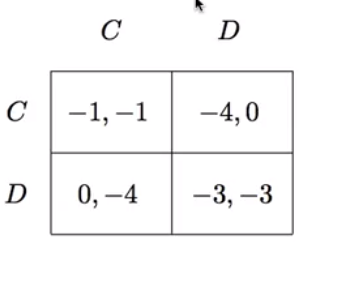
\includegraphics[width = 8cm, height = 8cm]{IMG_001.png} \\
    \emph{Figure 1}
\end{center}
Such that
\begin{center}
    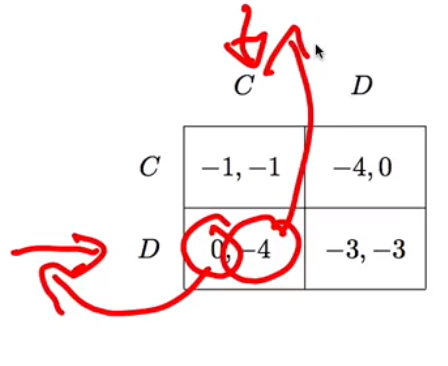
\includegraphics[width = 8cm, height = 8cm]{IMG_002.png} \\
    \emph{Figure 2}
\end{center}
\vskip 0.1in
\emph{A Large Collective Action Game}
\vskip 0.1in
\textbf{Players:} \(N = \{1, ..., 10,000,000\}\).
\vskip 0.05in
\textbf{Action Set:} for player \(i: A_{i} = \{\text{Revolt, Not} \}\).
\vskip 0.05in 
\textbf{Utility Function:} for player \(i\):
\begin{itemize}
    \item \(u_{i}(a) = 1\) if \(\{j: a_{j}\} = \text{Revolt} \geq 2,000,000\).
    \item \(u_{i}(a) = -1\) if \(\{j: a_{j}\} = \text{Revolt} < 2,000,000\) and \(a_{i} = \) Revolt.
    \item \(u_{i}(a) = 0\) if \(\{j: a_{j}\} = \text{Revolt} < 2,000,000\) and \(a_{i} = \) Not.
\end{itemize}

\section{Examples of Games}

There are plenty of other examples of what games could be played. Take for example the \textbf{Prisoner's Dilemma} is any game such that the Normal Form is:
\begin{center}
    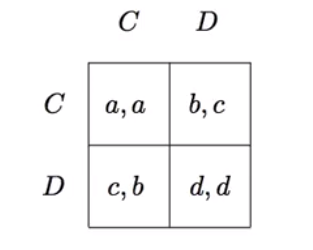
\includegraphics[width = 8cm, height = 6cm]{IMG_003.png} \\
    \emph{Figure 3}
\end{center}
Where \(c > a > d > b\).
\vskip 0.1in
\emph{Games of Pure Competition}
\vskip 0.1in
Think of games that exist purely due to basis of competition. Then players have \textbf{exactly opposed} interests. By the standard of this type of game, there must be precisely two players (otherwise they can't have exactly opposed interests - factual). The standard of pure competition also states for all action profiles \(a \in A\), \(u_{1}(a) + u_{2}(a) = c\) for some constant \(c\) (The special case for this is the \emph{zero sum} instances). Thus, intuitively, we only need to store a utility function for \emph{one} player (in a sense, we only have to think of one player's interests). For example, take the game of matching pennies: One player wants a match, the other player wants a mismatch. Thus, the matrix we would create would be: 
\begin{center}
    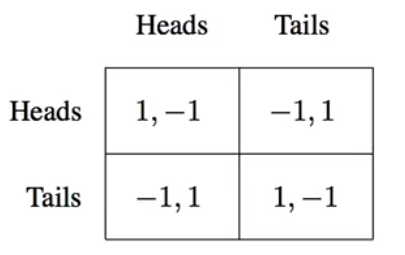
\includegraphics[width = 8cm, height = 6cm]{IMG_004.png} \\
    \emph{Figure 4}
\end{center}
It's clear that whenever one player wins, then the other loses; thus, pure competition is the type of game being played. Another example would be if we were to play Rock-Paper-Scissors: 
\begin{center}
    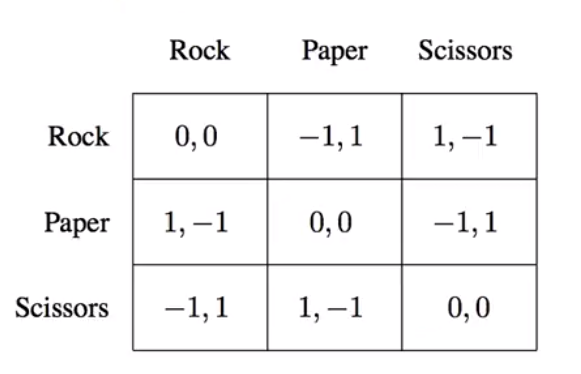
\includegraphics[width = 8cm, height = 6cm]{IMG_005.png} \\
    \emph{Figure 5}
\end{center}
Again, it's clear that this is pure competition due to one player being direct opposition of the other. Either they win, lose, or no result (Rock-Rock = 0-0). 
\vskip 0.1in
\emph{Games of Cooperation}
\vskip 0.1in
Now think of games that exist on the basis of competition. Players of these games have \textbf{exactly the same} interests. In these games, there's almost no conflict s.t. all players want the same things. The mathematical representation of the utility function is as follows:
\begin{align}
    \forall a \in A, \forall i, j, u_{i}(a) = u_{j}(a).
\end{align}
In these situations, we often write such games with a single payoff per cell. Then the question arises when we define "cooperative" games; \emph{why are such games "non-cooperative"?} To better understand the idea of cooperative games, let's define an example called "Coordination Game". The question is what side of the sidewalk should you walk on? So if you walk on left, while the other player walks on the left - then of course you reach a collision, otherwise if you walk on the right while they walk on the left, then clearly nothing happens and you continue to move forward. This is defined in Standard Form as:
\begin{center}
    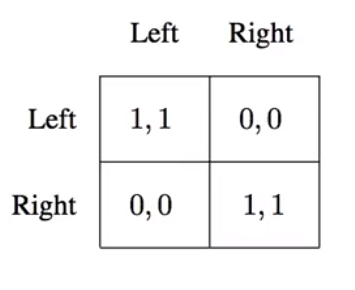
\includegraphics[width = 8cm, height = 6cm]{IMG_006.png} \\
    \emph{Figure 6}
\end{center}
\vskip 0.1in
\emph{General Games}
\vskip 0.1in
Some of the most interesting games thus combine elements of both \emph{cooperation} \textbf{and} \emph{competition}. Take for example that it's date night and you have a Battle/Action/War film (B) and Romantic film (F) to choose from. Of course if you and your significant other decide to go to different movies, then neither are satisfied. But in any case, when one person chooses one movie then both are satisfied to some degree, but one lesser than the other. The Standard Form looks like:
\begin{center}
    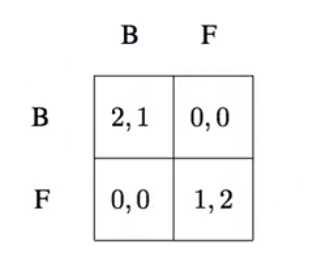
\includegraphics[width = 8cm, height = 6cm]{IMG_007.png} \\
    \emph{Figure 7}
\end{center}

\section{Nash-Equilibrium Intro}

Before going into Nash-Equilibrium, we must first analyze Keynes' Beauty Contest Game. This beauty contest game can be modeled by using the stock market as an example. For example, say you hold stock and the price is rising for that stock (so far so good!) But you believe that the price is too high to be justified by the company that holds that stock. Now you would like to sell this stock, but would like to wait until the price is almost at it's peak. You would like to get out of the market \emph{just before the other investors do}. So then the questions formulate: \emph{How will they act? What should you do in response?}
\vskip 0.1in
The basic ingredients of Nash-Equilibrium is that we must have some prediction of what the other players are doing, and then choosing the optimal strategy in response to that. The stylized version of Keynes' Beauty Contest then emerges. 
\vskip 0.1in
\emph{Keynes' Beauty Contest Game: The Stylized Version}
\vskip 0.1in
The stylized version is one in which each of the player's name an integer between 1 and 100. The player who chooses the integer closest to two thirds of the \emph{average} integer wins the prize, while all the other players get nothing. Ties are then broken uniformly at random.

\section{Strategic Reasoning}

So now let's take the example of the Beauty Contest Game from above. The strategic reasoning that emerges begs the questions: What will other players do? What should I do in response? Each player that \emph{best responds} to the \emph{others} is known as the Nash-Equilibrium. So now we must figure out what the Nash-Equilibrium of this game is:
\vskip 0.1in
\emph{Solving the Beauty Contest Game}
\vskip 0.1in
Suppose a player believes that the average integer (including his/her own integer) is \(X\). Then that player's optimal strategy is to say the closest integer to \(\frac{2}{3}X\). \(X\) has to be less than \(100\), so the optimal strategy of any player has to be no more than \(67\). If \(X\) is no more than \(67\), then the optimal strategy of any player has to be no more than \(\frac{2}{3}67\). If \(X\) is no more than \(\frac{2}{3}67\), then the optimal strategy of any player has to be no more than \((\frac{2}{3})^{2}67\). Iterating these simulations, then the unique Nash Equilibrium of this game is for every player to announce 1! Then every player would win the prize, but this also assumes that every player is \textbf{rational} with their decisions. The following histogram shows an example of when this game was played an the corresponding winners: 
\begin{center}
    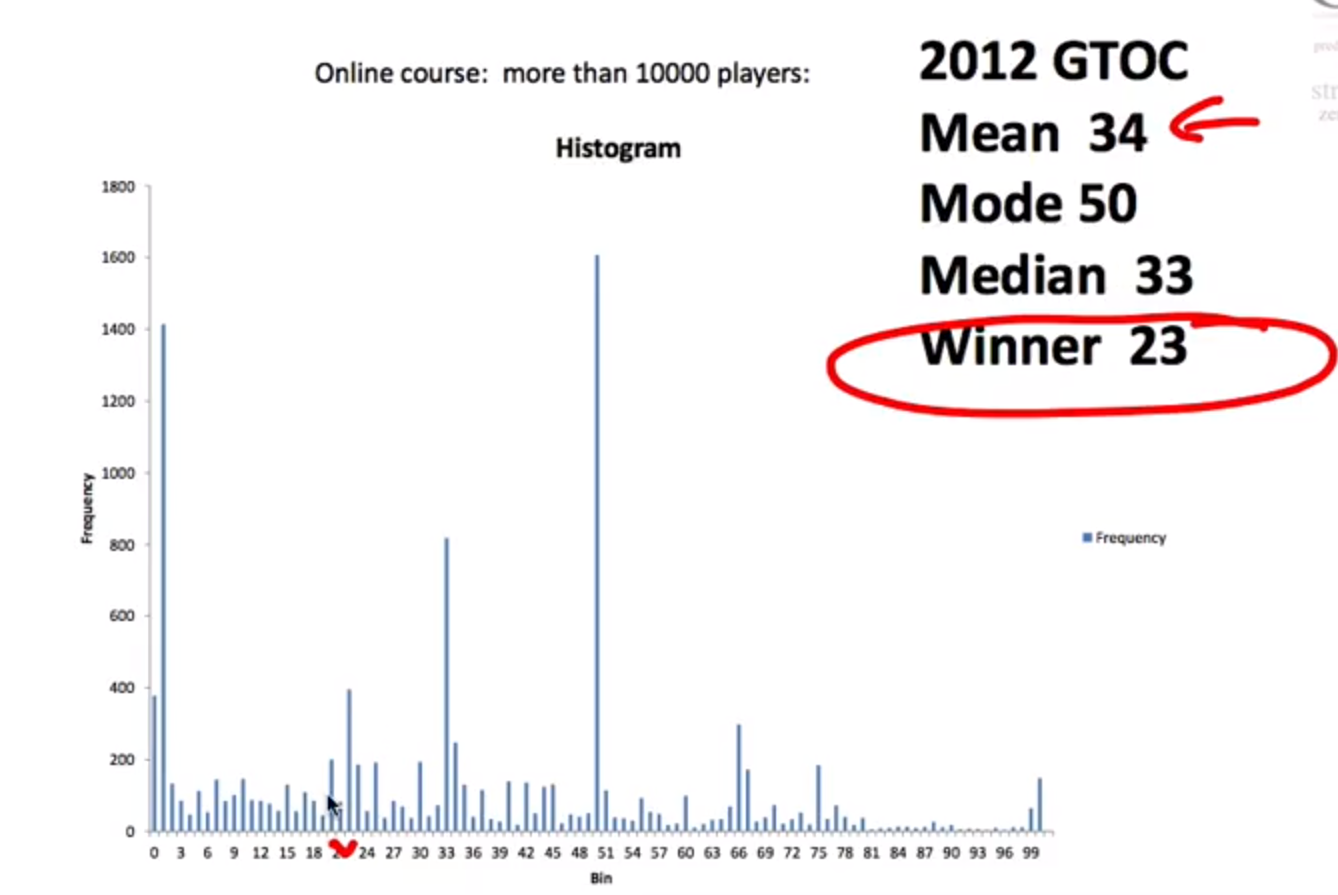
\includegraphics[width = 8cm, height = 8cm]{IMG_008.png} \\
    \emph{Figure 8}
\end{center}
Now say that all the players know the previous outcome of the "first round" and have them play a "second round" of the exact same game. Then the following histogram is an example of the outcome: 
\begin{center}
    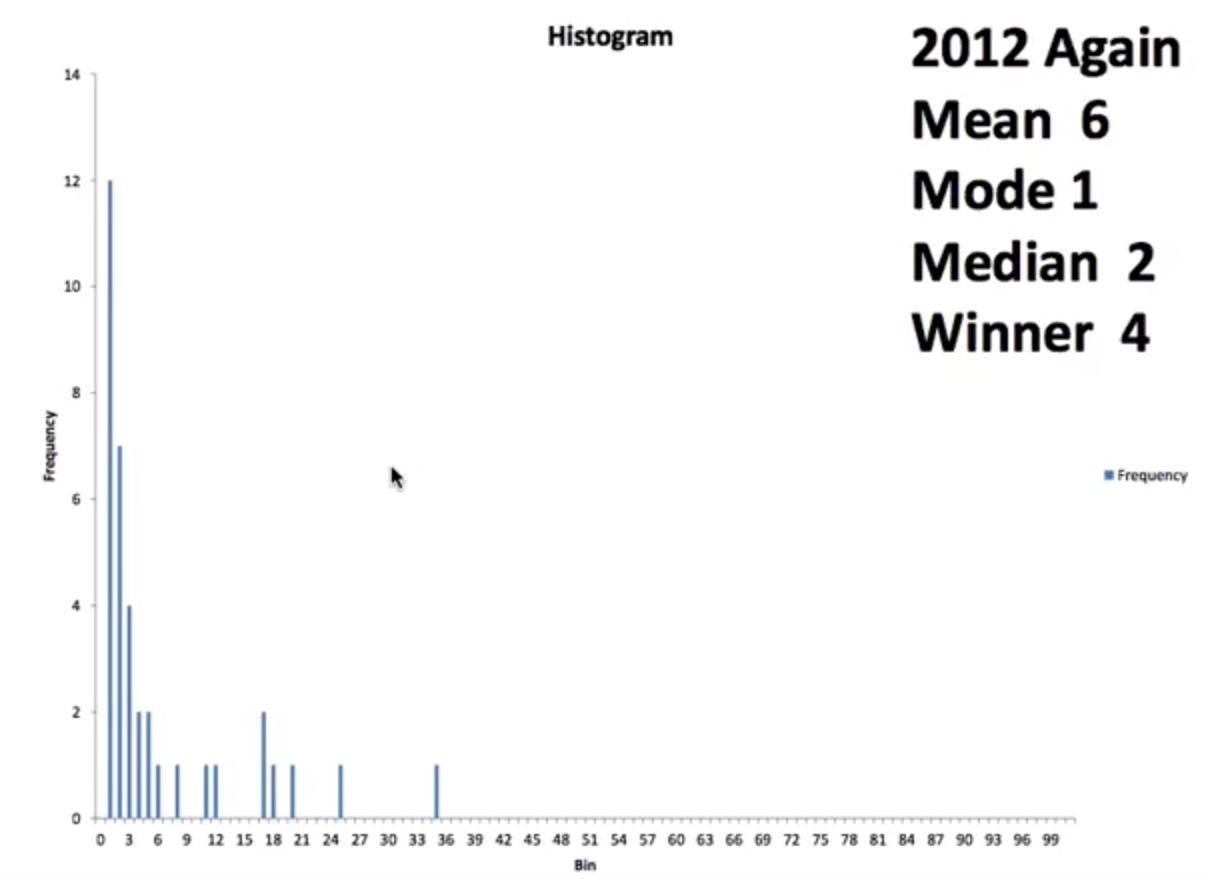
\includegraphics[width = 8cm, height = 8cm]{IMG_009.png} \\
    \emph{Figure 9}
\end{center}
It's clear that the "Winner" solutions as well as the "Median" is approaching 1. Thus, we can conclusively state that 1 is the stable Nash Equilibrium of this game even through testing (rather than only theory). The Nash Equilibrium is a consistent list of actions, in which each player's actions maximizes his or her payoff given the actions to the others. Lastly, the Nash Equilibrium is a self-consistent or stable profile. 
\vskip 0.1in
\emph{Summary of Nash Equilibrium}
\vskip 0.1in
\begin{itemize}
    \item Each player's action maximizes his or her payoff given the actions of the others.
    \item Nobody has an incentive to \emph{deviate} from their action if an equilibrium profile is played.
    \item Someone has an incentive to \emph{deviate} from a profile of actions that do \emph{not} form an equilibrium. 
\end{itemize}
Finally, the questions stand: Should we expect equilibria to be played? Or should we expect non-equilibria to be played? And the answer is that we should expect non-equilibria to be played (clearly shown in \emph{Figure 8}). 

\section{Best Response and Nash Equilibrium}

\emph{Best Response (BR)}
\vskip 0.1in
If you knew what everyone else was going to do, it would be simple to pick your own action. Let \(a_{-i} = \langle a_{1}, ..., a_{i-1}, a_{i+1}, ..., a_{n}\rangle\), s.t. \(a_{i}\) is your own action, and \(a_{-i}\) is the vector containing all other actions possible. Now by this definition, \(a = (a_{-i}, a_{i})\). And the definition of the Best Response (BR) in mathematical notation is:
\begin{align}
    a_{i}^{*} \in BR(a_{-i}) \text{ iff } \forall a_{i} \in A_{i}, u_{i}(a_{i}^{*}, a_{-i}) \geq u_{i}(a_{i}, a_{-i}).
\end{align}

\vskip 0.1in
\emph{Nash Equilibrium}
\vskip 0.1in
In this scenario, really, no agent knows what the others will do. What can we say about the actions that will occur? For an idea, look for \emph{stable} action profiles. The definition of the Nash Equilibrium in mathematical notation is:
\begin{align}
    a = \langle a_{1}, ..., a_{n}\rangle \textbf{ is a ("pure strategy") \emph{Nash equilibium} iff } \forall i, a_{i} \in BR(a_{-i}).
\end{align}

\section{Nash Equilibrium of Example Games}

Now let's revist the specific game concepts that we outlined earlier, starting with the Prisoners' Dilemma (with actual numbers this time):
\begin{center}
    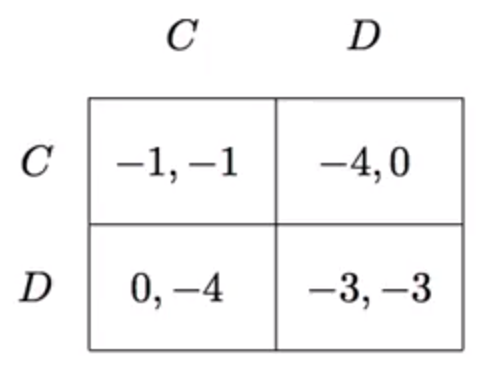
\includegraphics[width = 8cm, height = 8cm]{IMG_010.png} \\
    \emph{Figure 10}
\end{center}
In this example, the Nash equilibrium is to defect/not-cooperate no matter what the other prisoner does. The dominant strategy is also evident in that no matter what's happening, defecting will be the best outcome (D). 
\vskip 0.1in 
Now take the game of cooperation where we're walking on the sidewalk. Then the game has 2 Nash equilibria of whenever the other person walks to the left, you also walk to the left. Whenever the person walks to the right, you also walk to right. This is fairly straight-forward and explicit in that there's no room for any other kind of interpretation. 
\vskip 0.1in
Now take the example of the game in which there's both competition and cooperation as in the Date Night example. Then the Nash equilibria is both seeing the either of the movies. The difference between this and the game of pure coorperation, is that one person gains more satisfaction than the other based on which movie is being seen. So the goal for \emph{you} is to see the movie you personally prefer to see.
\vskip 0.1in
Lastly, take the example of the Matching Game where there was pure competition. The best response of individuals is interesting in this game because the responses are cyclical on the basis of who's answer could be potentially chosen, and the Nash equilibria is in 4 different places due to the changes in best response. A visual of this Standard Form is outlined below:
\begin{center}
    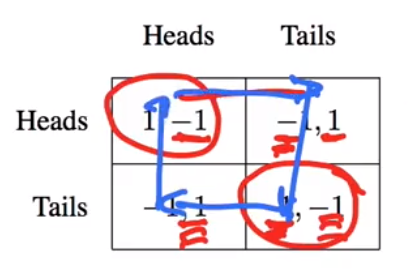
\includegraphics[width = 8cm, height = 8cm]{IMG_011.png} \\
    \emph{Figure 11}
\end{center}

\section{Dominant Strategies}

\emph{Domination}
\vskip 0.1in
Let \(s_{i}\) and \(s_{i}^{'}\) be two strategies for player \(i\), and let \(S_{-i}\) be the set of all possible strategy profiles for the other players. You might be asking yourself, "What's a strategy?" And for now we'll simply define this as just choosing an action (known as "pure strategy"), but this definition will become more refined as the course progresses. So then we first define \textbf{strict dominance}:
\begin{align}
    s_{i} \text{\emph{ strictly dominates }} s_{i}^{'} \text{ if } \forall s_{-i} \in S_{-i}, u_{i}(s_{i}, s_{-i}) > u_{i}(s_{i}^{'}, s_{-i}).
\end{align}
Whereas, we define \textbf{weak dominance} as:
\begin{align}
    s_{i} \text{\emph{ very weakly dominates }} s_{i}^{'} \text{ if } \forall s_{-i} \in S_{-i}, u_{i}(s_{i}, s_{-i}) \geq u_{i}(s_{i}^{'}, s_{-i}).
\end{align}
\vskip 0.1in
\emph{Equilibria and Dominance}
\vskip 0.1in
So when we have a situation where one strategy dominates all other strategies, we say that strategy is \emph{dominant}. A strategy profile consisting of dominant strategies for every player must then be a Nash equilibrium. As an aside, an equilibrium in strictly dominant strategies must be unique (due to the strict inequality, rather than the opportunity of equality - as in very weak dominance).
\vskip 0.05in
For example, take the prisoner example from earlier. If we go through case-analysis for the dominant strategy of Player 1 (the row player), then it's clear that the best strategy (no matter Player 2's choice of action) is to be defiant. This is clearly outlined in the following Standard Matrix:
\begin{center}
    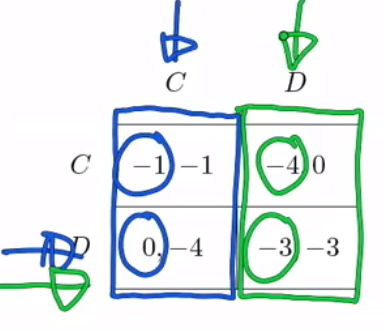
\includegraphics[width = 8cm, height = 8cm]{IMG_012.png} \\
    \emph{Figure 12}
\end{center}
Thus, we can also conclude through a similar case analysis, that Player 2's dominant strategy is also always be defiant, no matter Player 1's action. Hence we call the act of defiance for both prisoners as the strictly dominant strategies. 

\section{Pareto Optimality}

\emph{Analyzing Games}
\vskip 0.1in
We've defined some canonical games, and thought about how to play them. Now let's examine the games from the \emph{outside}. From the point of view of an outside observer, can some outcomes of a game be said to be \emph{better} than others? The issue we run into is that we \emph{cannot} say one agent's interests are more important than another agent's interests; imagine as though you're trying to find the revenue-maximizing outcome when you don't know what currency is used to express each agent's payoff. So then this begs the question: \emph{Are there still ways to prefer one outcome to another?}
\vskip 0.1in
\emph{Pareto Optimality}
\vskip 0.1in
Now we have an \textbf{idea}: sometimes, one outcome \(o\) is at least as good for every agent as another outcome \(o^{'}\), and there is some agent who strictly prefers \(o\) to \(o^{'}\). Thus, in this case it seems reasonable to say that \(o\) is better than \(o^{'}\) although, this is not necessarily true! In this case (of the resultant outcomes between \(o\) and \(o^{'}\)) we say that \(o\) \textbf{Pareto-dominates} \(o^{'}\). Thus the definition emerges:
\begin{center}
    \text{An outcome \(o^{*}\) is \textbf{Pareto-optimal} if there is no other outcome that Pareto-dominates it.}
    \emph{Definition}
\end{center}
\vskip 0.05in
Can a game have more than one Pareto-optimal outcome? The answer is yes, yes it can. For example, take the example in which we're cooperatively walking on a sidewalk. The Pareto-optimal outcomes are where both of us walk to the left, or both of us walk to the right. Hence there are 2 Pareto-optimal outcomes to this game. Does every game have at least one Pareto-optimal outcome? The answer is yes. Every game must have the very best option for the players participating. 
\vskip 0.1in
If we take the example of the Matching Heads-Tails Game; the Pareto-optimal outcome is any of the 4 outcomes, because this is a zero-sum game (this Pareto-optimal outcome is common in zero-sum games). When we take the example of the Prisoner Dilemma, then the Pareto-optimal outcome is actually when either both prisoners cooperate, and/or when one prisoner cooperates. Now this game is a \emph{dilemma} because the Pareto-optimal outcomes are different to the strictly dominant/Nash equilibrium solution to the game. Thus, Pareto-optimality does \emph{not} necessarily have to be the same as the Nash equilibria. 
\end{document}
